% !TeX root = ../main.tex
% !TeX spelling = en_GB
% !TeX program = pdflatex

\chapter{Results}
\label{chap:results}

The contents of this chapter are also found in Paper III. This result shown here can be seen as the answers to research question RQ4, and partly RQ5 from \Cref{chap:intro}.

\section{Measurement of Polymer Microspheres}

Four NIST calibrated distributions of microspheres, approximately 5, 10, 20 and 50 µm in diameter were used, resulting in four different measured size distributions. All images were saved and visually inspected, resulting in some measurement outliers due to clogging of smaller particles or contamination of small particles among larger. The outliers that were identified as not of the real distribution are not included in the result shown. Histograms of the measurement can be found in Figure \ref{fig:Histograms}. A summary of the result is shown in Table \ref{tab:poly_meas}.

\begin{figure}[ht]
\centering
\begin{subfigure}{.5\textwidth}
  \centering
  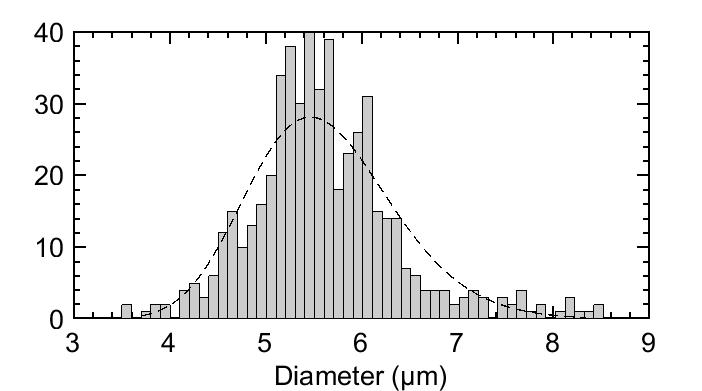
\includegraphics[width=1\linewidth]{figures/Images/Measurement1_5um}
  \subcaption{Distribution I.}
  \label{fig:Meas1_5um}
\end{subfigure}
\begin{subfigure}{.49\textwidth}
  \centering
  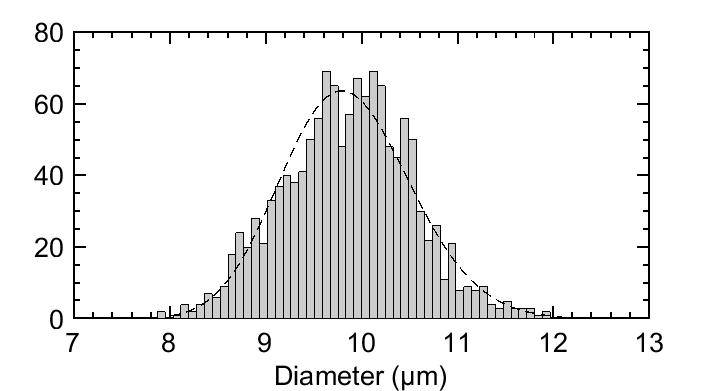
\includegraphics[width=1\linewidth]{figures/Images/Measurement1_10um}
  \subcaption{Distribution II.}
  \label{fig:Meas1_10um}
\end{subfigure}
\begin{subfigure}{.5\textwidth}
  \centering
  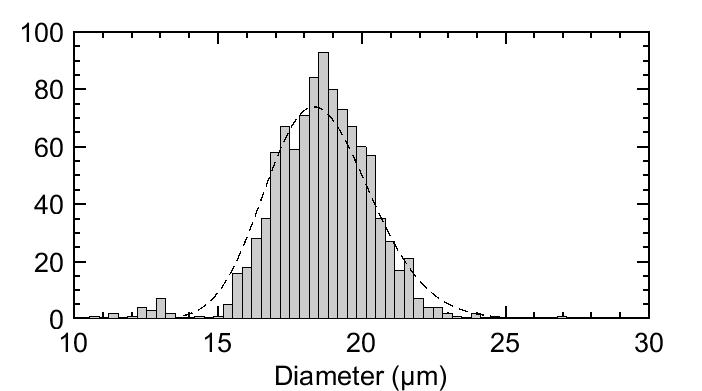
\includegraphics[width=1\linewidth]{figures/Images/Measurement1_20um}
  \subcaption{Distribution III.}
  \label{fig:Meas1_20um}
\end{subfigure}
\begin{subfigure}{.49\textwidth}
  \centering
  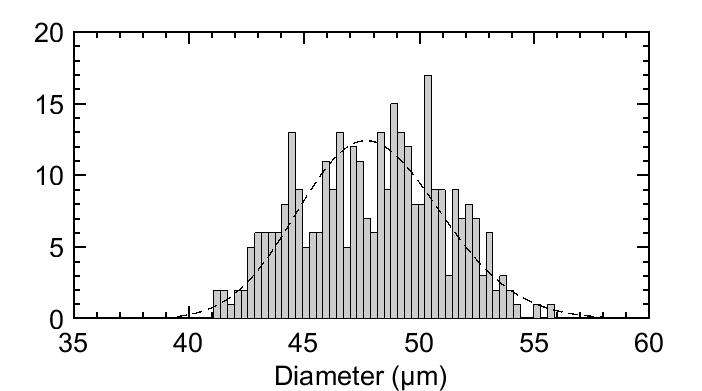
\includegraphics[width=1\linewidth]{figures/Images/Measurement1_50um}
  \subcaption{Distribution IV.}
  \label{fig:Meas1_50um}
\end{subfigure}
\caption{Histograms of the four measured distributions. The dashed line is a fitted  lognormal of the weighted distribution.}
\label{fig:Histograms}
\end{figure}

\begin{table}[ht]
\centering
\begin{tabular}{p{0.32\linewidth} p{0.14\linewidth} p{0.14\linewidth} p{0.14\linewidth} p{0.14\linewidth}}
\hline
\textbf{Distribution} & \textbf{I} & \textbf{II} & \textbf{III} & \textbf{IV}\\
\hline
Stated mean diam. & 5.3\newline \hspace{1em} ($\pm$ 0.3) & 10.3\newline \hspace{1em} ($\pm$ 0.4) & 19.1\newline \hspace{1em} ($\pm$ 0.7) & 49.4\newline \hspace{1em} ($\pm$ 1.6) \\
Measured mean diam. & 5.6 & 9.9 & 18.6 & 48.0 \\
\hline
Stated std. dev. & 0.5 & 0.9 & 1.7 & 3.5 \\
Measured std. dev. & 0.77 & 0.67 & 1.7 & 3.1 \\
\hline
\end{tabular}
\caption{Summary of the result from the measurement of NIST certified microspheres. All values are in µm.}
\label{tab:poly_meas}
\end{table}

\section{Comparison of DII and CDP Data}

Figure \ref{fig:0228-0301_MVD_DIIvsCDP} shows the MVD measured by the CDP compared with the DII. The least squares method applied on the data set results in a slope of 0.77 and a very small offset of -0.3 µm. Ideally, if both instruments were measuring the true diameter, the slope here would be equal to 1. A straight line with a slope that is not equal to 1 means that there is a systematic difference between the CDP and the DII in the size measurement.

\begin{figure}[ht]
\centering
\begin{subfigure}{.85\textwidth}
  \centering
  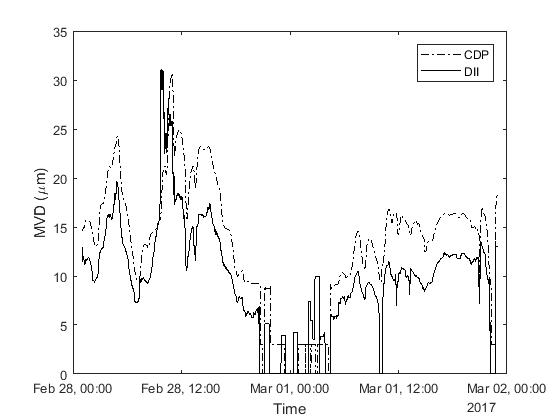
\includegraphics[width=1\linewidth]{figures/0228-0301/30min_mvd_CDP_DII_170228-170301_19212_0LpartDII_214646_0LpartCDP}
  \subcaption{MVD vs. time}
  \label{fig:0228-0301_MVDvstime}
\end{subfigure}%

\begin{subfigure}{.85\textwidth}
  \centering
  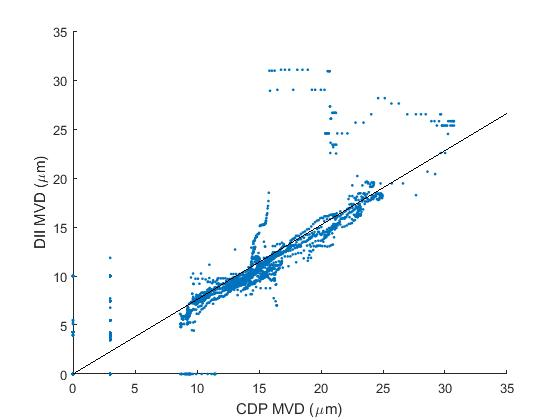
\includegraphics[width=1\linewidth]{figures/0228-0301/Mvdquote_DII-CDP_17022801-17030123_2760min_leastsquare0_7682}
  \subcaption{MVD measured by DII versus CDP}
  \label{fig:0228-0301_MVD_DIIvsCDP}
\end{subfigure}
\caption{MVD minute values measured by the DII and the CDP for 46 hours on 28-02-2017--01-03-2017.}
\label{fig:0228-0301_mvd}
\end{figure}

We compare the instruments by studying the data from 28 February to 1 March. See Figure \ref{fig:0228-0301_lwc} and \ref{fig:0228-0301_mvd}. Figure \ref{fig:0228-0301_LWC_DIIvsCDP} shows the LWC measured by the CDP compared with LWC measured by the DII. Using the least square method on the whole data set gives an average quote of 0.27. The quote is drawn in the plot as a straight line from the origin. Here too, the ideal case is a straight line with the slope equal to 1. The difference is discussed in \Cref{sec:systemdiff}.

\begin{figure}[ht]
\centering
\begin{subfigure}{.85\textwidth}
  \centering
  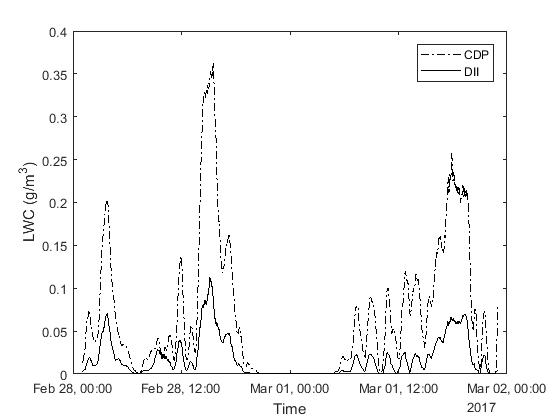
\includegraphics[width=1\linewidth]{figures/0228-0301/30min_lwc_CDP_DII_170228-170301_19212_0LpartDII_214646_0LpartCDP}
  \subcaption{LWC as a function of time}
  \label{fig:0228-0301_LWCvstime}
\end{subfigure}%

\begin{subfigure}{.85\textwidth}
  \centering
  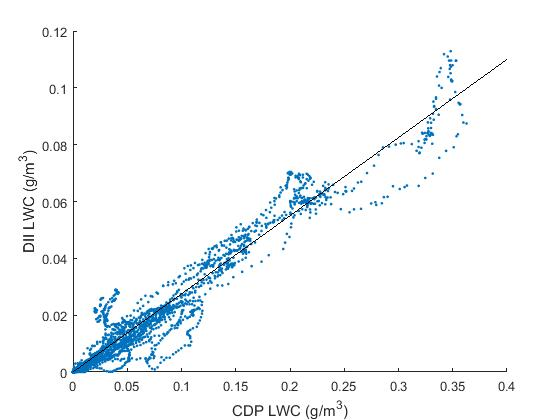
\includegraphics[width=1\linewidth]{figures/0228-0301/Lwcquote_DII-CDP_17022801-17030123_2760min_leastsquare0_2742}
  \subcaption{LWC measured by DII versus CDP}
  \label{fig:0228-0301_LWC_DIIvsCDP}
\end{subfigure}
\caption{LWC measured by the DII and the CDP for 46 hours on 28-02-2017--01-03-2017.}
\label{fig:0228-0301_lwc}
\end{figure}

\clearpage
The quote between the LWC values of the two instruments is plotted together with the wind speed in Figure \ref{fig:0228-0301_WSvslwcquote}. The least square average is plotted as a horizontal line at 3.65 (CDP LWC/DII LWC). The logarithmic scale is cropped with 238 quote values above 100 and 121 values below 0.1 out of a total of 2760.

\begin{figure}[ht]
  \centering
  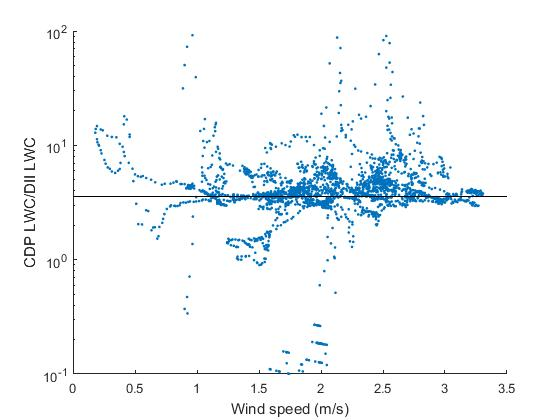
\includegraphics[width=0.85\linewidth]{figures/0228-0301/Relation_between_lwcquote_and_wind_speed_17022801-17030123}
\caption{Relation between the wind speed and the quote between the LWC measured by the CDP and the DII. The vertical scale is cropped at 1 and 100. 238 values are above 100 and 121 below 1 out of a total of 2760.}
\label{fig:0228-0301_WSvslwcquote}
\end{figure}

\clearpage
\section{Comparison of Measured and Modeled Data}

Figure \ref{fig:161211_mvd_lwc} shows the LWC and the MVD from the two instruments compared with the data from the HARMONIE-AROME model at 500 m resolution. The fog lasted for about 19 hours on 12-11-2016. The difference between the two instruments follows the same systematic pattern during this specific measurement, as in all the other observations. The HARMONIE-AROME model data of the LWC follows the general data of the LWC but fails to detect the large increase in LWC between 05:00 and 12:00. The predicted MVD of the model is closer to the actual values of the DII than the CDP.

\begin{figure}[ht]
\centering
\begin{subfigure}[t]{.85\textwidth}
  \centering
  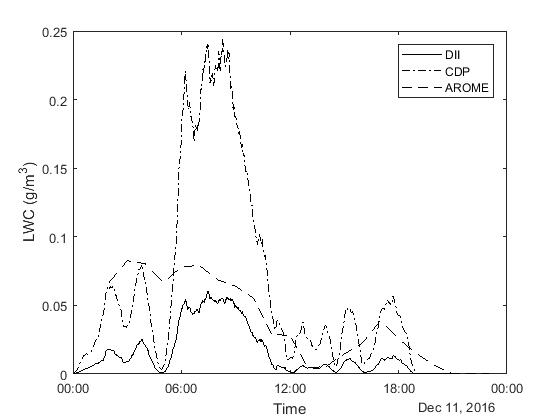
\includegraphics[width=1\linewidth]{figures/161211/30min_lwc_CDP_DII_SMHI_161211_adjusted}
  \subcaption{LWC vs. time}
  \label{fig:161211_LWCvstime}
\end{subfigure}%

\begin{subfigure}[t]{.85\textwidth}
  \centering
  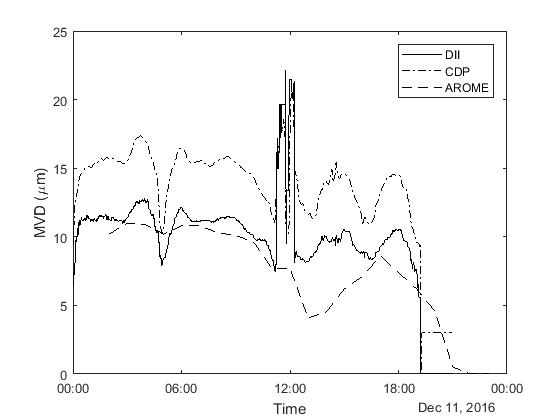
\includegraphics[width=1\linewidth]{figures/161211/30min_mvd_CDP_DII_SMHI_161211_adjusted}
  \subcaption{MVD vs. time}
  \label{fig:161211_MVDvstime}
\end{subfigure}
\caption{LWC and MVD measured by the DII and the CDP 11-12-2016. HARMONIE-AROME model data using 500 meter resolution. }
\label{fig:161211_mvd_lwc}
\end{figure}

\clearpage
Figure \ref{fig:0203-0206_lwc_mvd} shows the result from measurement 03-02-2017--06-02-2017. Unfortunately, no data from the CDP was saved at this point, due to a full memory. The double spike in the MVD diagram \ref{fig:0203-0206_MVDvstime} at 04:17 and 04:41 on 05-02-2017 is mainly caused by two droplets, 51 and 74 µm (see Figure \ref{fig:170505_0441_droplet}) in combination with a number of large droplets between 30 and 40 µm in diameter.

\begin{figure}[ht]
\centering
\begin{subfigure}[t]{.85\textwidth}
  \centering
  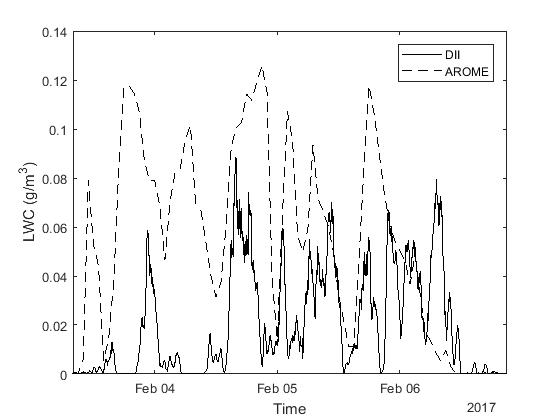
\includegraphics[width=1\linewidth]{figures/0203-0206/30min_lwc_foggy_smhi_170203-170206_86h}
  \subcaption{LWC vs. time.}
  \label{fig:0203-0206_LWCvstime}
\end{subfigure}%

\begin{subfigure}[t]{.85\textwidth}
  \centering
  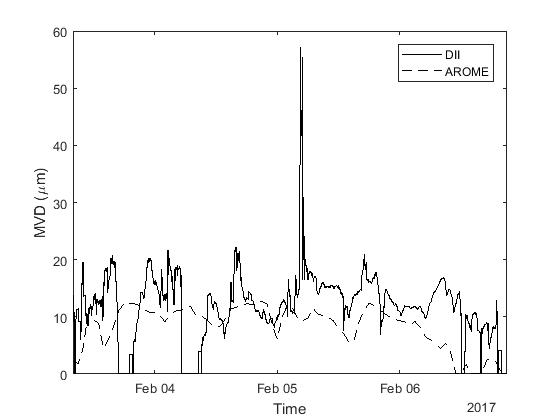
\includegraphics[width=1\linewidth]{figures/0203-0206/30min_mvd_foggy_smhi_170203-170206_86h}
  \subcaption{MVD vs. time.}
  \label{fig:0203-0206_MVDvstime}
\end{subfigure}
\caption{LWC and MVD measured 03-02-2017--06-02-2017 by the DII. HARMONIE-AROME model data using 2.5 km resolution, stored every 60 minutes.}
\label{fig:0203-0206_lwc_mvd}
\end{figure}

\begin{figure}[ht]
\centering
\begin{subfigure}[t]{.8\textwidth}
  \centering
  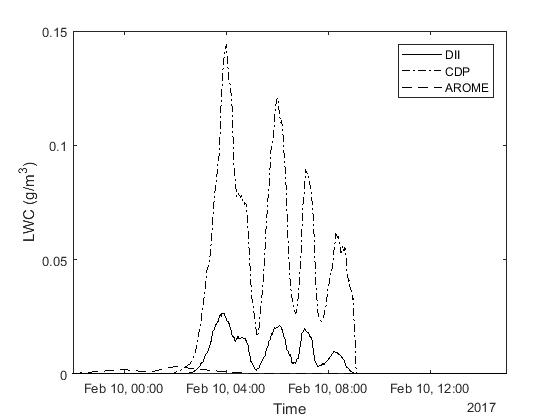
\includegraphics[width=1\linewidth]{figures/170210/30min_lwc_CDP_DII_SMHI_170210_2263part}
  \subcaption{LWC vs. time.}
  \label{fig:170210_LWCvstime}
\end{subfigure}%

\begin{subfigure}[t]{.8\textwidth}
  \centering
  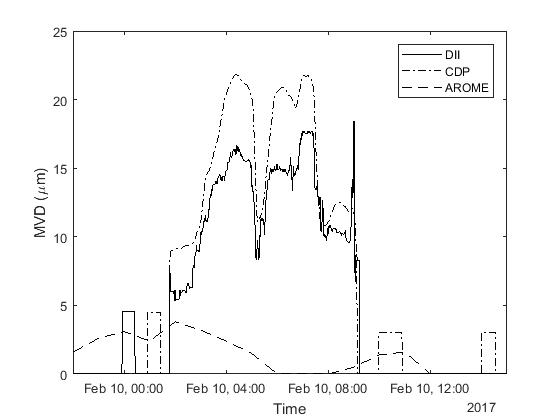
\includegraphics[width=1\linewidth]{figures/170210/30min_mvd_CDP_DII_SMHI_170210_2263part}
  \subcaption{MVD vs. time.}
  \label{fig:170210_MVDvstime}
\end{subfigure}
\caption{LWC and MVD measured by the DII and the CDP 10-02-2017. HARMONIE-AROME model data using 2.5 km resolution, stored every 60 minutes.}
\label{fig:170210_lwc_mvd}
\end{figure}

